
\subsection{Gini coefficient}

As mentioned in Section~\ref{giniKindaSucks}, the Gini coefficient is not the
ideal measure of inequality for our apocalyptic model. Nonetheless, it is
illustrative to see how it varies with respect to the ER $\lambda$ parameter.
Figure~\ref{fig:giniVsLambda} depicts the Gini computed \textit{at the onset
of stage 3} (before starvation) versus $\lambda$, and confirms that...
% Will, finish this paragraph.

\begin{figure}[hb]
\centering
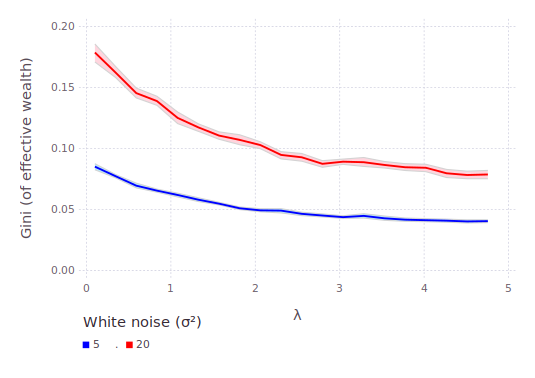
\includegraphics[width=\columnwidth]{figures/giniVsLambda.png}
\caption{The average Gini coefficient, computed before the onset of starvation,
for various values of the ER $\lambda$ connectivity parameter.}
\label{fig:giniVsLambda}
\end{figure}

% Will's text and plot showing Gini coefficient (pre-stage-3) decreases with λ

\subsection{Life expectancy}

% Plots from 7/12 showing you best get in a proto if lambda and white noise 
%   are high


% Wealth histogram is steady ?

